\documentclass[a4paper,12pt,twoside]{article}




%-------------------------------------------
%	CHARACTER ENCODING
%-------------------------------------------
\usepackage[utf8]{inputenc}

%-------------------------------------------
%	USEFUL COMMANDS
%-------------------------------------------

%-------------------------------------------
%	PACKAGES
%-------------------------------------------
\usepackage[english]{babel}

\usepackage{sectsty}

\usepackage{titlesec}

\usepackage{mathtools}

%------------------------------------------------
\usepackage{array,multirow}
\usepackage{booktabs}
%------------------------------------------------
\usepackage[dvipsnames]{xcolor}
%------------------------------------------------
\usepackage{textcomp}
\usepackage{enumitem}
\usepackage[load-configurations = abbreviations]{siunitx}
% \sisetup{locale = FR, range-phrase={ \`{a} }, list-final-separator={ et }, list-pair-separator={ et }, detect-all}
\usepackage{float,sidecap}
%------------------------------------------------
\usepackage[tracking]{microtype}
% \usepackage{mathptmx} % Corpus font
% \usepackage{newtxtext}
% \usepackage{newtxmath}
\usepackage{fourier}
\DeclareMathAlphabet{\mathcal}{OMS}{cmsy}{m}{n}
\usepackage[condensed]{roboto}
%\renewcommand{\sfdefault}{fvs} % Lato for 1st page and section titles fla
%\linespread{1.025}
%------------------------------------------------
\usepackage{import}
%\usepackage[final]{pdfpages}
\usepackage{graphicx}

%------------------------------------------------
\usepackage[a4paper]{geometry}
\usepackage[format=hang,font=small,labelfont={sf,bf},labelsep=endash]{caption}
\geometry{top=2.54cm, bottom=2.5cm, left=2.54cm , right=2.54cm}
%------------------------------------------------
\usepackage[T1]{fontenc}
%------------------------------------------------
\usepackage{fancyhdr}
\pagestyle{fancy}
\renewcommand{\sectionmark}[1]{\markright{\MakeUppercase{\thesection.\ #1}}}

\fancyhf{}
\fancyhead[LE,RO]{}
\fancyhead[RE,LO]{\rightmark}
\fancyfoot[CE,CO]{}
\fancyfoot[LE,RO]{\thepage}

%------------------------------------------------
\setlist{noitemsep}


%------------------------------------------------
\graphicspath{{illustrations/}{../illustrations/}}
%\allsectionsfont{\sffamily}
%\frenchbsetup{og = «, fg = »}
%\urlstyle{sf}

%-----------------------------------------------
\usepackage{xcolor} % Required for specifying colors by name
\definecolor{ocre}{RGB}{52,177,201} % Define the orange color used for highlighting throughout the book
\definecolor{blackout}{RGB}{0,0,0}

\usepackage{titlesec}
% use \llap if you want to align text section with left textwidth
\makeatletter
\renewcommand{\@seccntformat}[1]{\textcolor{black!55}{\csname the#1\endcsname}\hspace{0.5em}}                    
\renewcommand{\section}{\@startsection{section}{1}{\z@}
{-2.5ex}
{0.5ex }
{\normalfont\Large\sffamily\bfseries}}

\renewcommand{\subsection}{\@startsection {subsection}{2}{\z@}
{-1.5ex}
{0.5ex}
{\large\sffamily\bfseries}}

\renewcommand{\subsubsection}{\@startsection {subsubsection}{3}{\z@}
{-2ex \@plus -0.1ex \@minus -.2ex}
{.2ex \@plus.2ex }
{\sffamily\bfseries}}

\renewcommand\paragraph{\@startsection{paragraph}{4}{\z@}
{-2ex \@plus-.2ex \@minus .2ex}
{.1ex}
{\sffamily\bfseries\itshape}}
\makeatother

% \titleformat{\section}
% {\sffamily\large\bfseries\uppercase}{\thesection}{.5em}{}

% \titlespacing{\section}{0pt}{1em}{0.5em}

\usepackage{titletoc} % Required for manipulating the table of contents
\contentsmargin{0cm} % Removes the default margin
% Chapter text styling
%\titlecontents{chapter}[1.25cm] % Indentation
%{\addvspace{15pt}\large\sffamily\bfseries} % Spacing and font options for chapters
%{\color{ocre!60}\contentslabel[\Large\thecontentslabel]{1.25cm}\color{ocre}} % Chapter number
%{}  
%{\color{ocre!60}\normalsize\sffamily\bfseries\;\titlerule*[.5pc]{.}\;\thecontentspage} % Page number

% Section text styling
%\titlecontents{section}[1.25cm] % Indentation
%{\addvspace{5pt}\sffamily\bfseries} % Spacing and font options for sections
%{\contentslabel[\thecontentslabel]{1.25cm}} % Section number
%{}
%{\sffamily\hfill\color{black}\thecontentspage} % Page number
%[]
\titlecontents{section}[0.5cm] % Indentation
{\addvspace{6pt}\large\sffamily\bfseries} % Spacing and font options for chapters
{\color{black!50}\contentslabel[\Large\thecontentslabel]{0.7cm}\color{black}} % Section number
{}  
{\color{black!50}\normalsize\sffamily\bfseries\;\titlerule*[.5pc]{}\;\thecontentspage} % Page number

% Subsection text styling
%\titlecontents{subsection}[1.25cm] % Indentation
%{\addvspace{5pt}\sffamily\small} % Spacing and font options for subsections
%{\contentslabel[\thecontentslabel]{1.25cm}} % Subsection number
%{}
%{\sffamily\;\titlerule*[.5pc]{.}\;\thecontentspage} % Page number
%[]

\titlecontents{subsection}[1.4cm] % Indentation
{\addvspace{3pt}\sffamily\bfseries} % Spacing and font options for subsections
{\color{black!50}\contentslabel[\thecontentslabel]{0.8cm}\color{black}} % Section number
{}
{\sffamily\bfseries\color{black!50}\;\titlerule*[.6pc]{.}\;\thecontentspage} % Page number
[]

% Subsubsection text styling
\titlecontents{subsubsection}[2.5cm] % Indentation
{\addvspace{1pt}\sffamily\small\bfseries} % Spacing and font options for subsubsections
{\color{black!50}\contentslabel[\thecontentslabel]{1cm}\color{black}} % Subsubsection number
{}
{\sffamily\bfseries\color{black!50}\;\titlerule*[.6pc]{.}\;\thecontentspage} % Page number
[]


% Document begins here
%-----------------------------------------------
\begin{document}
\renewcommand{\headheight}{14.5pt}
\renewcommand{\tablename}{Table}
\renewcommand{\figurename}{Figure}

% Title page
\begin{titlepage}

\newcommand{\HRule}{\rule{\linewidth}{0.5mm}} % Defines a new command for the horizontal lines, change thickness here


\center % Center everything on the page
%----------------------------------------------------------------------------------------
%	LOGO SECTION
%----------------------------------------------------------------------------------------

\includegraphics[width=5cm]{logo_automatique}
\hfill

\includegraphics[width=5cm]{epfl}\\[4.5cm]

%----------------------------------------------------------------------------------------
%	HEADING SECTIONS
%----------------------------------------------------------------------------------------
%\normalfont\fontsize{26}{26}\sffamily\selectfont
%\textbf{Clustering the interstellar medium}\\
%{\LARGE Data Mining and Machine Learning in Astronomy}
%\textsc{ }\\[6cm]


%----------------------------------------------------------------------------------------
%	TITLE SECTION
%----------------------------------------------------------------------------------------

\HRule \\[0.2cm]
\sffamily
{\LARGE\bfseries \uppercase{Swing-up of a triple arm inverted pendulum}} \\[0.05cm]
{\Large\bfseries Master Semester Project}
\HRule \\[0.5cm]
 
%----------------------------------------------------------------------------------------
%	AUTHOR SECTION
%----------------------------------------------------------------------------------------

{\Large Laboratoire d'automatique}\\[0.1cm] % Name of your university/college
{\large Mechanical Engineering Faculty}\\[4.5cm] % Major heading such as course name

\begin{minipage}{0.45\textwidth}
    \begin{flushleft}
        \textbf{Author:}\\
        Frédéric NGUYEN
    \end{flushleft}
\end{minipage}
~
\begin{minipage}{0.45\textwidth}
    \begin{flushright}
        \textbf{Professor:} \\
        Dr. Philipe MÜLLHAUPT\\
        \textbf{Supervisor:}\\
        Ehsan SARSHARI
    \end{flushright}
\end{minipage}\\[2cm]

% If you don't want a supervisor, uncomment the two lines below and remove the section above
%\Large \emph{Author:}\\
%John \textsc{Smith}\\[3cm] % Your name

%----------------------------------------------------------------------------------------
%	DATE SECTION
%----------------------------------------------------------------------------------------
\vfill
{Lausanne, le 28 Décembre 2016}\\[1.5cm] % Date, change the \today to a set date if you want to be precise


 
%----------------------------------------------------------------------------------------

\vfill % Fill the rest of the page with whitespace

\end{titlepage}
\newpage
% Summary
\pagenumbering{roman}
\tableofcontents
\newpage

\pagenumbering{arabic}

%---------------------------------------------------------------
%	ABSTRACT
%---------------------------------------------------------------
\begin{abstract}
The swing-up of a triple pendulum.
In this report, the subject of the swing-up of a triple arm inverted pendulum is approached. The swing-up strategy is based on recording the motions of the triple pendulum and then replay the same movements but in the backward direction. The main focus of the report is on the modeling of the triple pendulum and the simulation of the swing-up phase by using the described strategy on MATLAB.

LQR controller
\end{abstract}

%---------------------------------------------------------------
%	INTRODUCTION
%---------------------------------------------------------------
\section{Introduction}\label{sec:intro} %ABSTRACT
The swing-up of a triple arm inverted pendulum is presented. The main focus of this semester project is to simulate a strategy for the swing-up of the pendulum. It is done to study the feasability of the strategy.
The goal of this project is to provide a solution for the swing-up of a triple arm inverted pendulum.

%---------------------------------------------------------------
%	PRINCIPLE OF THE SWING-UP STRATEGY
%---------------------------------------------------------------
\section{Principle of the swing-up strategy}
The main focus of this project is the swing-up phase of the pendulum. This phase consists in leading the cart of the triple pendulum from the stable equilibrium to an unstable equilibrium where all the arms are in the upright position.
\begin{figure}[ht]
	\centering
	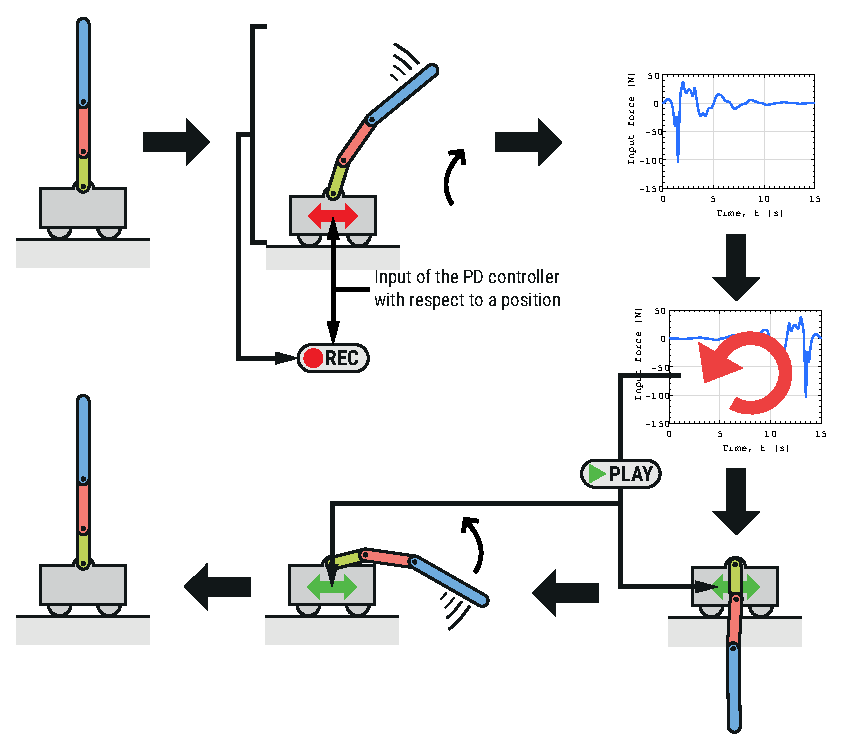
\includegraphics[width=0.9\textwidth]{principle_swingup}
	\caption{Principle of the swing-up strategy}
	\label{fig:swingup_strategy}
\end{figure}
%---------------------------------------------------------------
%	MODELING OF THE TRIPLE PENDULUM
%---------------------------------------------------------------
\section{Modeling of the triple pendulum}
For the purpose of this project, it is required to develop the equations of motion of the triple pendulum system. A \emph{Lagrangian approach} is used for the modeling of the triple pendulum in the following pages.

\subsection{Description of the triple pendulum}
The pendulum consists in three links which are linked together to a cart. The cart is the only actuated part of the system. The other parts are free to move in their degree of freedom. For each link, a length and a mass is defined. The links are supposed to be made of homogeneous material so the gravity center for each one are on the geometrical middle of each bars. The viscous friction in the bears of the cart and the links is not considered for the modeling of the triple pendulum.

A schematic representation of the system is showned in Figure \ref{fig:schematic_system}. The dispositions of the positions and angles, and the coordinate system are showned in Figure \ref{fig:schematic_system} and will be used for the modeling of the pendulum.
\begin{figure}[ht]
	\centering
	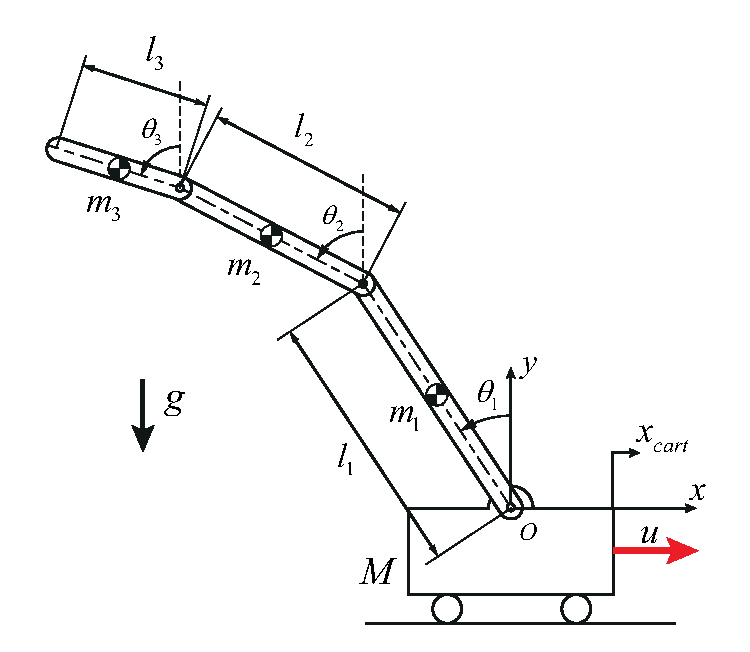
\includegraphics[width=11cm]{illustrations/schematic_system.eps}
	\caption{Triple arm inverted pendulum with assumed coordinate systems, dimensions and angles}
	\label{fig:schematic_system}
\end{figure}

Since there are four degrees of freedom for the system, there are also four generalized coordinates which are defined for this pendulum. The first one is the position of the cart $x_{cart}$ with respect to a reference. The last three generalized coordinates are the angles ($\theta_1$, $\theta_2$, $\theta_3$) of links at the joints. Their zero value are when the bars are in down position and they take their positives values when turning counterclockwise. The assignement of each degree of freedom to a generalized coordinate is according to the following:
\[
	x_{cart}\to q_1, \qquad \theta_1\to q_2, \qquad \theta_2\to q_3, \qquad \theta_3\to q_4
\]

The parameters of the system are given values in Table \ref{tab:parameters_system} and will be used for every simulation of the triple pendulum. The moments of inertia for each link is given by:
\[J_i = \frac{m_i\,l_i^2}{12}\]
\begin{table}[H]
	\centering
	\caption{Parameters for the following simulations}
	\label{tab:parameters_system}
	\begin{tabular}{@{}lll@{}}
		\toprule
		Parameter  & Value  & Unit                         \\ \midrule
		$m_{cart}$ & 1      & kg                           \\
		$m_1$      & 0.5    & kg                           \\
		$m_2$      & 0.5    & kg                           \\
		$m_3$      & 0.5    & kg                           \\
		$l_1$      & 1      & m                            \\
		$l_2$      & 1      & m                            \\
		$l_3$      & 1      & m                            \\
		$J_1$      & 0.0416 & \si{\kilo\gram\square\metre} \\
		$J_2$      & 0.0416 & \si{\kilo\gram\square\metre} \\
		$J_3$      & 0.0416 & \si{\kilo\gram\square\metre} \\
		$g$        & 9.81   & \si{m\per\square\second}     \\ \bottomrule
	\end{tabular}
\end{table}

\subsection{Mathematical model}
After defining the coordinate system and the generalized coordinates, the core of the modeling takes place here. The equations of motion for the system are derived from Lagrange's equations with a generalized force:
\begin{equation} \label{equ:Lagrange_motions}
	\frac{\text{d}}{\text{d}t} \left(\frac{\partial \mathcal{L}}{\partial \dot q_i}\right) - \frac{\partial \mathcal{L}}{\partial q_i} = u_i
	\quad \text{with}\ i=1,2,3,4
\end{equation}
Knowing that there is only one force input which exert to the cart, the different $u_i$ are defined such as $u_1 = u$ and $u_i = 0$ for $i=2,3,4$. To derive these equations of motion, the Lagrangian of the triple pendulum needs to be founded:
\begin{equation}
	\mathcal{L} = \mathcal{T} - \mathcal{V}
\end{equation}
where $\mathcal{T}$ is the kinetic energy and $\mathcal{V}$ the potential energy. Furthermore, the vectors from the origin of the coordinate system to the center of mass of each arms are defined by:
\[
	\mathbf{p}_1 =
	\begin{bmatrix}
		x_{cart} - l_1 \sin(\theta_1)/2 \\
		l_1 \cos(\theta_1)/2
	\end{bmatrix}
\]
\[
	\mathbf{p}_2 =
	\begin{bmatrix}
		x_{cart} - l_1 \sin(\theta_1) - l_2 \sin(\theta_2)/2 \\
		l_1 \cos(\theta_1) + l_2 \cos(\theta_2)/2
	\end{bmatrix}
\]
\[
	\mathbf{p}_3 =
	\begin{bmatrix}
		x_{cart} - l_1 \sin(\theta_1) - l_2 \sin(\theta_2) - l_3 \sin(\theta_3)/2 \\
		l_1 \cos(\theta_1) + l_2 \cos(\theta_2) + l_3 \cos(\theta_3)/2
	\end{bmatrix}
\]
The reasoning for deriving kinetic and potential energies is borrowed from \cite{}. The kinetic energy of the whole system is given by:
\begin{equation}
	\mathcal{T} = \frac{1}{2} m_{cart}\, \dot x_{cart}^2 +
		\frac{1}{2} \sum_{i=1}^{3} m_i \mathbf{\dot p}_i^T \mathbf{\dot p}_i +
		\frac{1}{2} \sum_{i=1}^{3} J_i\, \dot\theta_i^2
\end{equation}
The potential energy is computed with the $y$ components of each vector $\mathbf{p}_i$. Hence it is given by:
\begin{equation}
	\mathcal{V} = g \cdot \sum_{i=1}^3 m_i\, \mathbf{p}_{i,y}
\end{equation}

\subsection{Resolving the differential equations}

\subsection{Verification of the Lagrange model}


%---------------------------------------------------------------
%	SWING6UP OF THE TRIPLE PENDULUM
%---------------------------------------------------------------
\section{Swing-up of the triple pendulum}

\subsection{Generation of a downward trajectory}

\subsection{Simulation swing-up of the triple pendulum}

\subsection{Analysis}

%---------------------------------------------------------------
%	IMPLEMENTATION OF THE LQR STABILIZATION
%---------------------------------------------------------------
\section{Implementation of the LQR stabilization}
\subsection{Theory of the LQR regulator}

\subsection{Linearization of the equation of motion}
%---------------------------------------------------------------
%	CONCLUSION
%---------------------------------------------------------------
\section{Conclusion}

\end{document}
